\documentclass[12pt, a4paper]{article}

% ── Packages ──────────────────────────────────────────────────────────────────
\usepackage[margin=2.5cm]{geometry}
\usepackage{amsmath, amssymb}
\usepackage{graphicx}
\usepackage{booktabs}
\usepackage{array}
\usepackage{caption}
\usepackage{subcaption}
\usepackage[numbers,sort&compress]{natbib}  % Vancouver numbered citations
\usepackage{setspace}
\usepackage{parskip}
\usepackage{xcolor}
\usepackage{float}
\usepackage{tabularx}
\usepackage{multirow}
\usepackage{hyperref}   % load AFTER natbib
\hypersetup{
    colorlinks=true,
    linkcolor=blue!70!black,
    citecolor=blue!70!black,
    urlcolor=blue!70!black
}

% Abstract on same page as title: tighten title block spacing
\usepackage{titling}
\setlength{\droptitle}{-2em}
\pretitle{\begin{center}\large\bfseries}
\posttitle{\end{center}\vspace{-0.5em}}
\preauthor{\begin{center}\small}
\postauthor{\end{center}\vspace{-1em}}
\predate{\begin{center}\small}
\postdate{\end{center}\vspace{0.5em}}

\onehalfspacing

% ── Title block ───────────────────────────────────────────────────────────────
\title{Predicting Survival of Heart Failure Patients Using Machine Learning:
A Comparative Study of Traditional and Deep Learning Approaches}

\author{
    Shixian Qiu\\
    \small Medical AI Research Group\\
    \small \texttt{15812405499@163.com}
}

\date{\today}

% ══════════════════════════════════════════════════════════════════════════════
\begin{document}
\maketitle
\thispagestyle{empty}

% ── Abstract ──────────────────────────────────────────────────────────────────
\begin{abstract}
\noindent
\textbf{Background:} Heart failure (HF) is a leading cause of morbidity and 
mortality worldwide, affecting approximately 64 million people globally. 
Accurate prediction of patient survival during follow-up periods is critical 
for clinical decision-making and resource allocation.

\noindent
\textbf{Methods:} We analyzed a publicly available dataset of 299 heart failure 
patients collected at the Faisalabad Institute of Cardiology (Pakistan, 2015), 
comprising 13 clinical features. After exploratory data analysis and 
standardization, we applied four machine learning classifiers—Logistic 
Regression, Random Forest, XGBoost, and a Multilayer Perceptron (MLP)—to 
predict all-cause mortality. Feature importance was assessed via both Welch's 
$t$-test and Random Forest importance scores. Model performance was evaluated 
using accuracy, precision, recall, F1 score, and area under the receiver 
operating characteristic curve (AUC).

\noindent
\textbf{Results:} Random Forest achieved the best overall performance 
(AUC\,=\,0.897, Accuracy\,=\,0.850, F1\,=\,0.727), followed by XGBoost 
(AUC\,=\,0.849). Feature ranking consistently identified follow-up time, 
serum creatinine, and ejection fraction as the top three predictors of 
mortality. The deep learning MLP model showed comparatively lower performance 
(AUC\,=\,0.745), likely due to limited sample size.

\noindent
\textbf{Conclusions:} Machine learning models, particularly Random Forest, 
can effectively predict heart failure patient survival from routine clinical 
records. Serum creatinine and ejection fraction emerge as the most clinically 
actionable predictors, consistent with prior literature. These findings support 
the integration of machine learning tools into clinical prognostic workflows.

\medskip
\noindent\textbf{Keywords:} Heart failure; Survival prediction; Machine 
learning; Random Forest; XGBoost; Ejection fraction; Serum creatinine; 
ROC curve; Feature importance
\end{abstract}

% \newpage
% \tableofcontents
% \newpage

% ══════════════════════════════════════════════════════════════════════════════
\newpage
\section{Introduction}
\label{sec:intro}

Cardiovascular diseases (CVDs) are the leading cause of death globally, 
accounting for approximately 17.9 million deaths per year \cite{who2021}. 
Heart failure (HF), a clinical syndrome in which the heart is unable to pump 
sufficient blood to meet the body's metabolic demands, represents one of the 
most prevalent and costly manifestations of CVD \cite{virani2021}. The global 
prevalence of HF is estimated at 64 million individuals, with a five-year 
mortality rate exceeding 50\%—comparable to many malignancies \cite{groenewegen2020}.

The accurate prediction of short-term mortality in HF patients remains a 
formidable clinical challenge. Traditional risk stratification tools, such as 
the New York Heart Association (NYHA) functional classification, are largely 
subjective and fail to reliably quantify individual risk \cite{raphael2007}. 
Electronic health records (EHRs) now routinely capture a rich array of 
clinical, biochemical, and demographic variables that may encode prognostic 
information not readily apparent to clinicians. Machine learning (ML) 
algorithms are particularly well-suited to extract non-linear patterns from 
such high-dimensional data, offering a promising avenue for data-driven 
prognostication \cite{chicco2020}.

Several prior studies have applied ML to HF survival prediction. Chicco and 
Jurman \cite{chicco2020} demonstrated that serum creatinine and ejection 
fraction alone were sufficient to achieve competitive predictive performance 
using the same 299-patient dataset employed in the present work. Subsequent 
investigations have explored ensemble methods, deep learning architectures, 
and hybrid approaches, generally reporting AUC values in the range 
0.75--0.90 \cite{ahmad2017, hu2021}.

Despite this body of work, a comprehensive head-to-head comparison of 
traditional ML algorithms against a simple deep learning baseline—implemented 
with full transparency, reproducibility, and clinical interpretability—remains 
underrepresented in the literature. The present study addresses this gap by: 
(1) performing systematic exploratory data analysis (EDA) and feature 
engineering; (2) training and evaluating four classifiers spanning linear 
models, ensemble trees, gradient boosting, and neural networks; and 
(3) identifying the most clinically meaningful risk factors through both 
statistical testing and model-based importance ranking.

% ══════════════════════════════════════════════════════════════════════════════
\section{Materials and Methods}
\label{sec:methods}

\subsection{Dataset}

We used the publicly available Heart Failure Clinical Records dataset, 
originally collected by Ahmad et al.\ \cite{ahmad2017} from the 
Faisalabad Institute of Cardiology and the Allied Hospital, Faisalabad, 
Pakistan, during April–December 2015. The dataset contains medical records 
for 299 patients (194 male, 105 female) aged 40–95 years, all of whom had 
left ventricular systolic dysfunction and were classified as NYHA Class III 
or IV at baseline. The target variable, \texttt{DEATH\_EVENT}, is a binary 
indicator of all-cause mortality during the follow-up period 
(mean 130 days). Class distribution: 203 survivors (67.9\%) and 96 
deceased (32.1\%).

\subsection{Data Preprocessing}

\subsubsection{Exploratory Data Analysis}

Descriptive statistics (mean, standard deviation, quartiles) were computed 
for all 13 features. No missing values or duplicate records were identified. 
Binary features (\texttt{anaemia}, \texttt{diabetes}, 
\texttt{high\_blood\_pressure}, \texttt{sex}, \texttt{smoking}) were treated 
as categorical indicators and excluded from outlier analysis. Outlier 
detection for continuous features was performed using the interquartile range 
(IQR) method, with boundaries defined as:

\begin{equation}
    \text{Lower bound} = Q_1 - 1.5 \times \text{IQR}, \quad
    \text{Upper bound} = Q_3 + 1.5 \times \text{IQR}
    \label{eq:iqr}
\end{equation}

Outliers were retained rather than removed, as extreme values in clinical 
biochemistry (e.g., elevated serum creatinine, very low ejection fraction) 
frequently represent genuine pathophysiology rather than measurement error.

\subsubsection{Normalization}

All features were standardized to zero mean and unit variance using 
$z$-score normalization:

\begin{equation}
    z = \frac{x - \mu}{\sigma}
    \label{eq:zscore}
\end{equation}

where $\mu$ and $\sigma$ denote the training-set mean and standard deviation, 
respectively. This step is required for Logistic Regression and MLP, which 
are sensitive to feature scale. Random Forest and XGBoost, being tree-based 
methods, are scale-invariant; standardization was nonetheless applied 
uniformly to facilitate fair comparison.

\subsection{Feature Importance Analysis}

\subsubsection{Statistical Testing}

Group differences between survivors and deceased patients were evaluated 
using Welch's two-sample $t$-test (assuming unequal variances) for all 
continuous features. Features with $p < 0.05$ were considered statistically 
significant predictors of mortality.

\subsubsection{Random Forest Importance}

Feature importance scores were derived from a Random Forest classifier 
($n_\text{estimators} = 500$, \texttt{class\_weight} = ``balanced'') trained 
on the full feature set, using the mean decrease in impurity (MDI) criterion.

\subsection{Prediction Models}

The dataset was partitioned into training (80\%, $n=239$) and test 
(20\%, $n=60$) sets using stratified random splitting to preserve the 
class ratio. Four classifiers were evaluated:

\begin{enumerate}
    \item \textbf{Logistic Regression (LR):} A linear probabilistic 
    classifier modeling the log-odds of death. The binary cross-entropy 
    loss function is:
    \begin{equation}
        \mathcal{L}_\text{LR} = -\frac{1}{N}\sum_{i=1}^{N}
        \left[ y_i \log \hat{p}_i + (1-y_i)\log(1-\hat{p}_i) \right]
        \label{eq:logloss}
    \end{equation}
    where $y_i \in \{0,1\}$ is the true label and $\hat{p}_i$ is the 
    predicted probability of death. Class weights were balanced; 
    $L_2$ regularization was applied with \texttt{max\_iter}$=1000$.

    \item \textbf{Random Forest (RF):} An ensemble of 500 decision trees 
    with bootstrap aggregation (bagging). Class weights were set to 
    ``balanced'' to address class imbalance.

    \item \textbf{XGBoost:} A gradient boosting framework minimizing a 
    regularized objective. Hyperparameters: $n_\text{estimators}=300$, 
    \texttt{max\_depth}$=3$, \texttt{learning\_rate}$=0.05$, 
    \texttt{subsample}$=0.8$.

    \item \textbf{Multilayer Perceptron (MLP):} A fully-connected neural 
    network with two hidden layers of 32 and 16 neurons, ReLU activation, 
    Adam optimizer, and early stopping. The network minimizes the same 
    binary cross-entropy loss as Equation~\eqref{eq:logloss}.
\end{enumerate}

\subsection{Model Evaluation Metrics}

Model performance was assessed on the held-out test set using:

\begin{align}
    \text{Accuracy} &= \frac{TP + TN}{TP + TN + FP + FN} \label{eq:acc} \\[6pt]
    \text{Precision} &= \frac{TP}{TP + FP} \label{eq:prec} \\[6pt]
    \text{Recall} &= \frac{TP}{TP + FN} \label{eq:rec} \\[6pt]
    F_1 &= 2 \cdot \frac{\text{Precision} \times \text{Recall}}
                         {\text{Precision} + \text{Recall}} \label{eq:f1}
\end{align}

where $TP$, $TN$, $FP$, $FN$ denote true positives, true negatives, false 
positives, and false negatives, respectively. The area under the ROC curve 
(AUC) was computed as a threshold-independent summary of discriminative 
ability.

% ══════════════════════════════════════════════════════════════════════════════
\section{Results}
\label{sec:results}

\subsection{Descriptive Statistics and Class Distribution}

Table~\ref{tab:baseline} summarizes the baseline clinical characteristics 
of the study cohort, stratified by survival outcome. The deceased group was 
significantly older ($65.2 \pm 11.2$ vs.\ $58.8 \pm 11.9$ years, 
$p < 0.001$), had higher serum creatinine ($1.84 \pm 1.39$ vs.\ 
$1.18 \pm 0.73$ mg/dL, $p < 0.001$), and lower ejection fraction 
($33.5 \pm 12.6$ vs.\ $40.3 \pm 11.1$\%, $p < 0.001$).

\begin{table}[H]
\centering
\caption{Baseline clinical characteristics stratified by mortality outcome.
Values are mean $\pm$ SD for continuous variables or count (\%) for binary 
variables. $p$-values from Welch's $t$-test.}
\label{tab:baseline}
\renewcommand{\arraystretch}{1.35}
\begin{tabular}{lcccc}
\toprule
\textbf{Feature} & \textbf{Overall} & \textbf{Survived} & \textbf{Deceased} & \textbf{\textit{p}-value} \\
                 & ($n=299$)        & ($n=203$)          & ($n=96$)          &               \\
\midrule
Age (years)                  & $60.8 \pm 11.9$ & $58.8 \pm 11.9$ & $65.2 \pm 11.2$ & $<0.001$ \\
Ejection fraction (\%)       & $38.1 \pm 11.8$ & $40.3 \pm 11.1$ & $33.5 \pm 12.6$ & $<0.001$ \\
Serum creatinine (mg/dL)     & $1.39 \pm 1.03$ & $1.18 \pm 0.73$ & $1.84 \pm 1.39$ & $<0.001$ \\
Serum sodium (mEq/L)         & $136.6 \pm 4.4$ & $137.2 \pm 4.1$ & $135.4 \pm 4.8$ & $0.002$  \\
Creatinine phosphokinase (U/L) & $581.8 \pm 970.3$ & $540.1 \pm 908.0$ & $670.2 \pm 1081.8$ & $0.369$ \\
Platelets ($\times 10^3$/\textmu L) & $263.4 \pm 97.8$ & $266.7 \pm 96.9$ & $256.4 \pm 99.9$ & $0.399$ \\
Follow-up time (days)        & $130.3 \pm 77.6$ & $158.3 \pm 71.3$ & $70.9 \pm 60.5$ & $<0.001$ \\
\midrule
Anaemia, $n$ (\%)            & 129 (43.1)      & 83 (40.9)       & 46 (47.9)       & $0.253$  \\
Diabetes, $n$ (\%)           & 125 (41.8)      & 85 (41.9)       & 40 (41.7)       & $0.973$  \\
High blood pressure, $n$ (\%)& 105 (35.1)      & 66 (32.5)       & 39 (40.6)       & $0.171$  \\
Male sex, $n$ (\%)           & 194 (64.9)      & 133 (65.5)      & 61 (63.5)       & $0.741$  \\
Smoking, $n$ (\%)            & 96 (32.1)       & 66 (32.5)       & 30 (31.3)       & $0.828$  \\
\bottomrule
\end{tabular}
\end{table}

\subsection{Feature Importance}

Figure~\ref{fig:heatmap} presents the Pearson correlation heatmap across all 
13 clinical variables. Follow-up time showed the strongest correlation with 
\texttt{DEATH\_EVENT} ($r = -0.527$), followed by ejection fraction 
($r = -0.269$) and serum creatinine ($r = +0.294$). 

Figure~\ref{fig:importance} shows the Random Forest feature importance 
ranking. The top three features were: (1) follow-up time (0.358), 
(2) serum creatinine (0.162), and (3) ejection fraction (0.129). 
These rankings were concordant with the Welch's $t$-test results 
($p < 0.001$ for all three), providing cross-validated evidence 
for their prognostic relevance.

\begin{figure}[H]
    \centering
    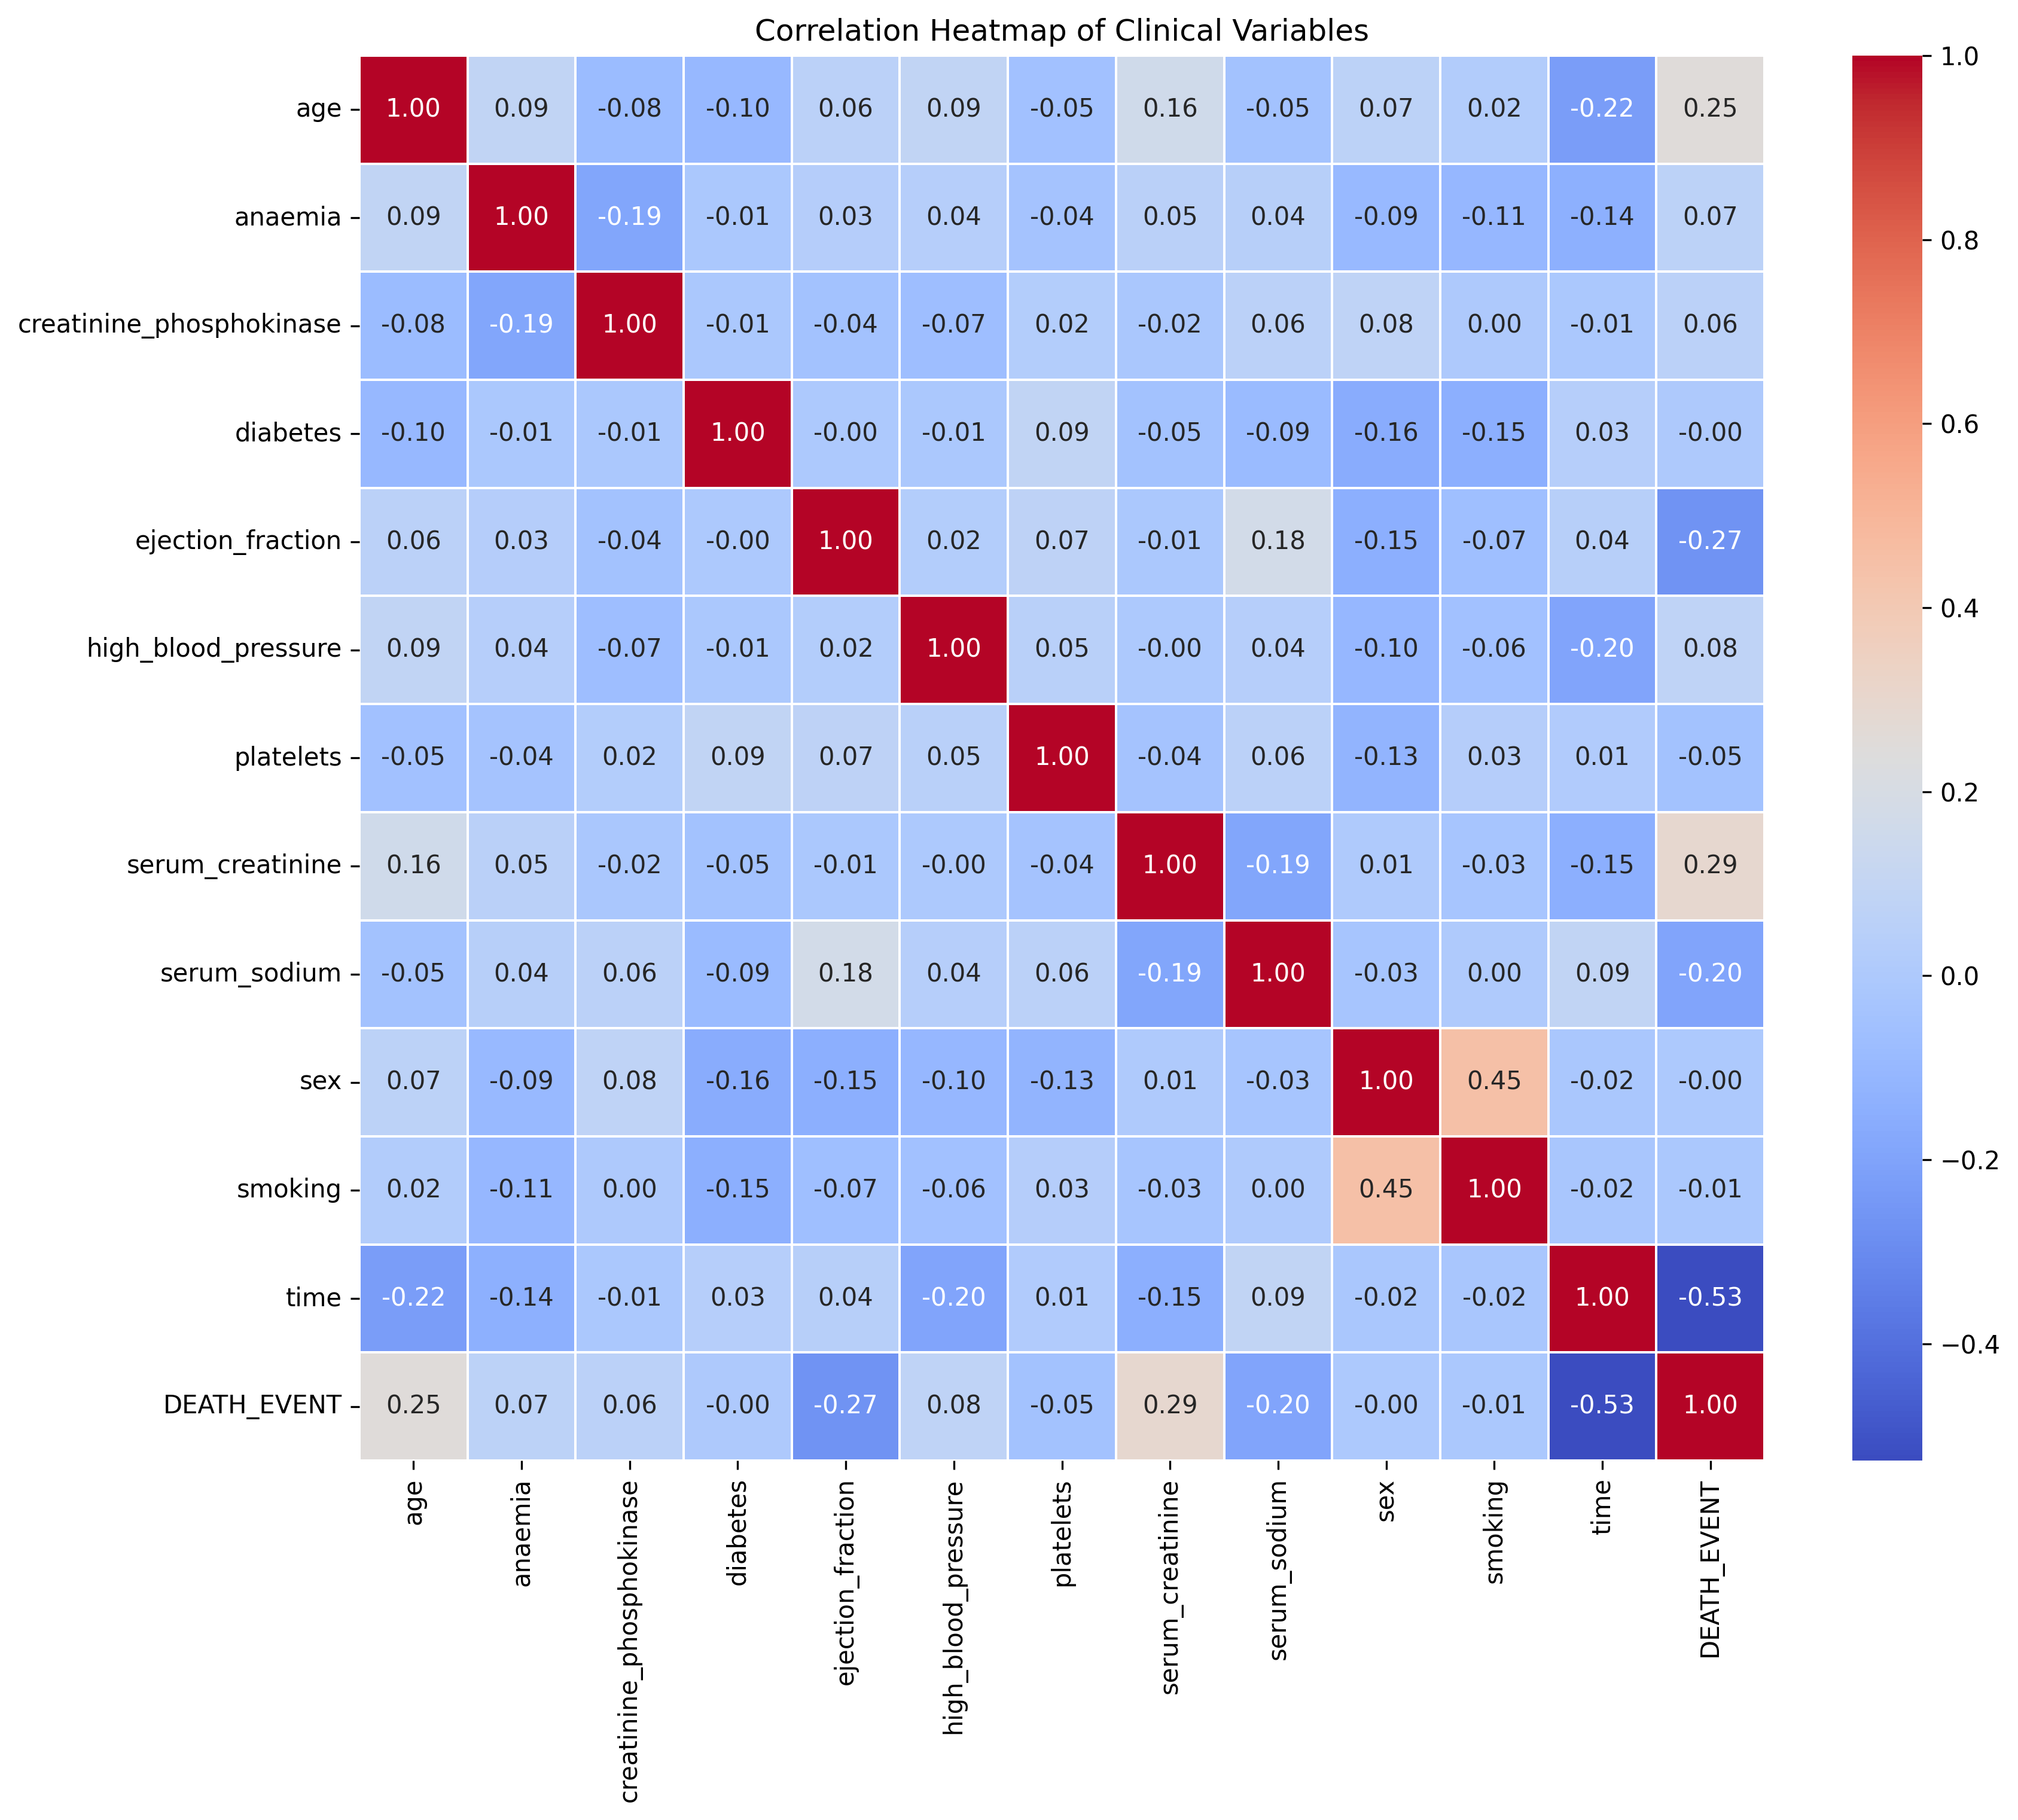
\includegraphics[width=0.90\textwidth]{heatmap.png}
    \caption{Pearson correlation heatmap of all 13 clinical features. 
    Colour intensity encodes correlation magnitude; red indicates positive 
    correlation and blue indicates negative correlation. \texttt{DEATH\_EVENT} 
    exhibits the strongest negative correlation with follow-up time 
    ($r = -0.527$) and ejection fraction ($r = -0.269$), and the strongest 
    positive correlation with serum creatinine ($r = +0.294$).}
    \label{fig:heatmap}
\end{figure}

\begin{figure}[H]
    \centering
    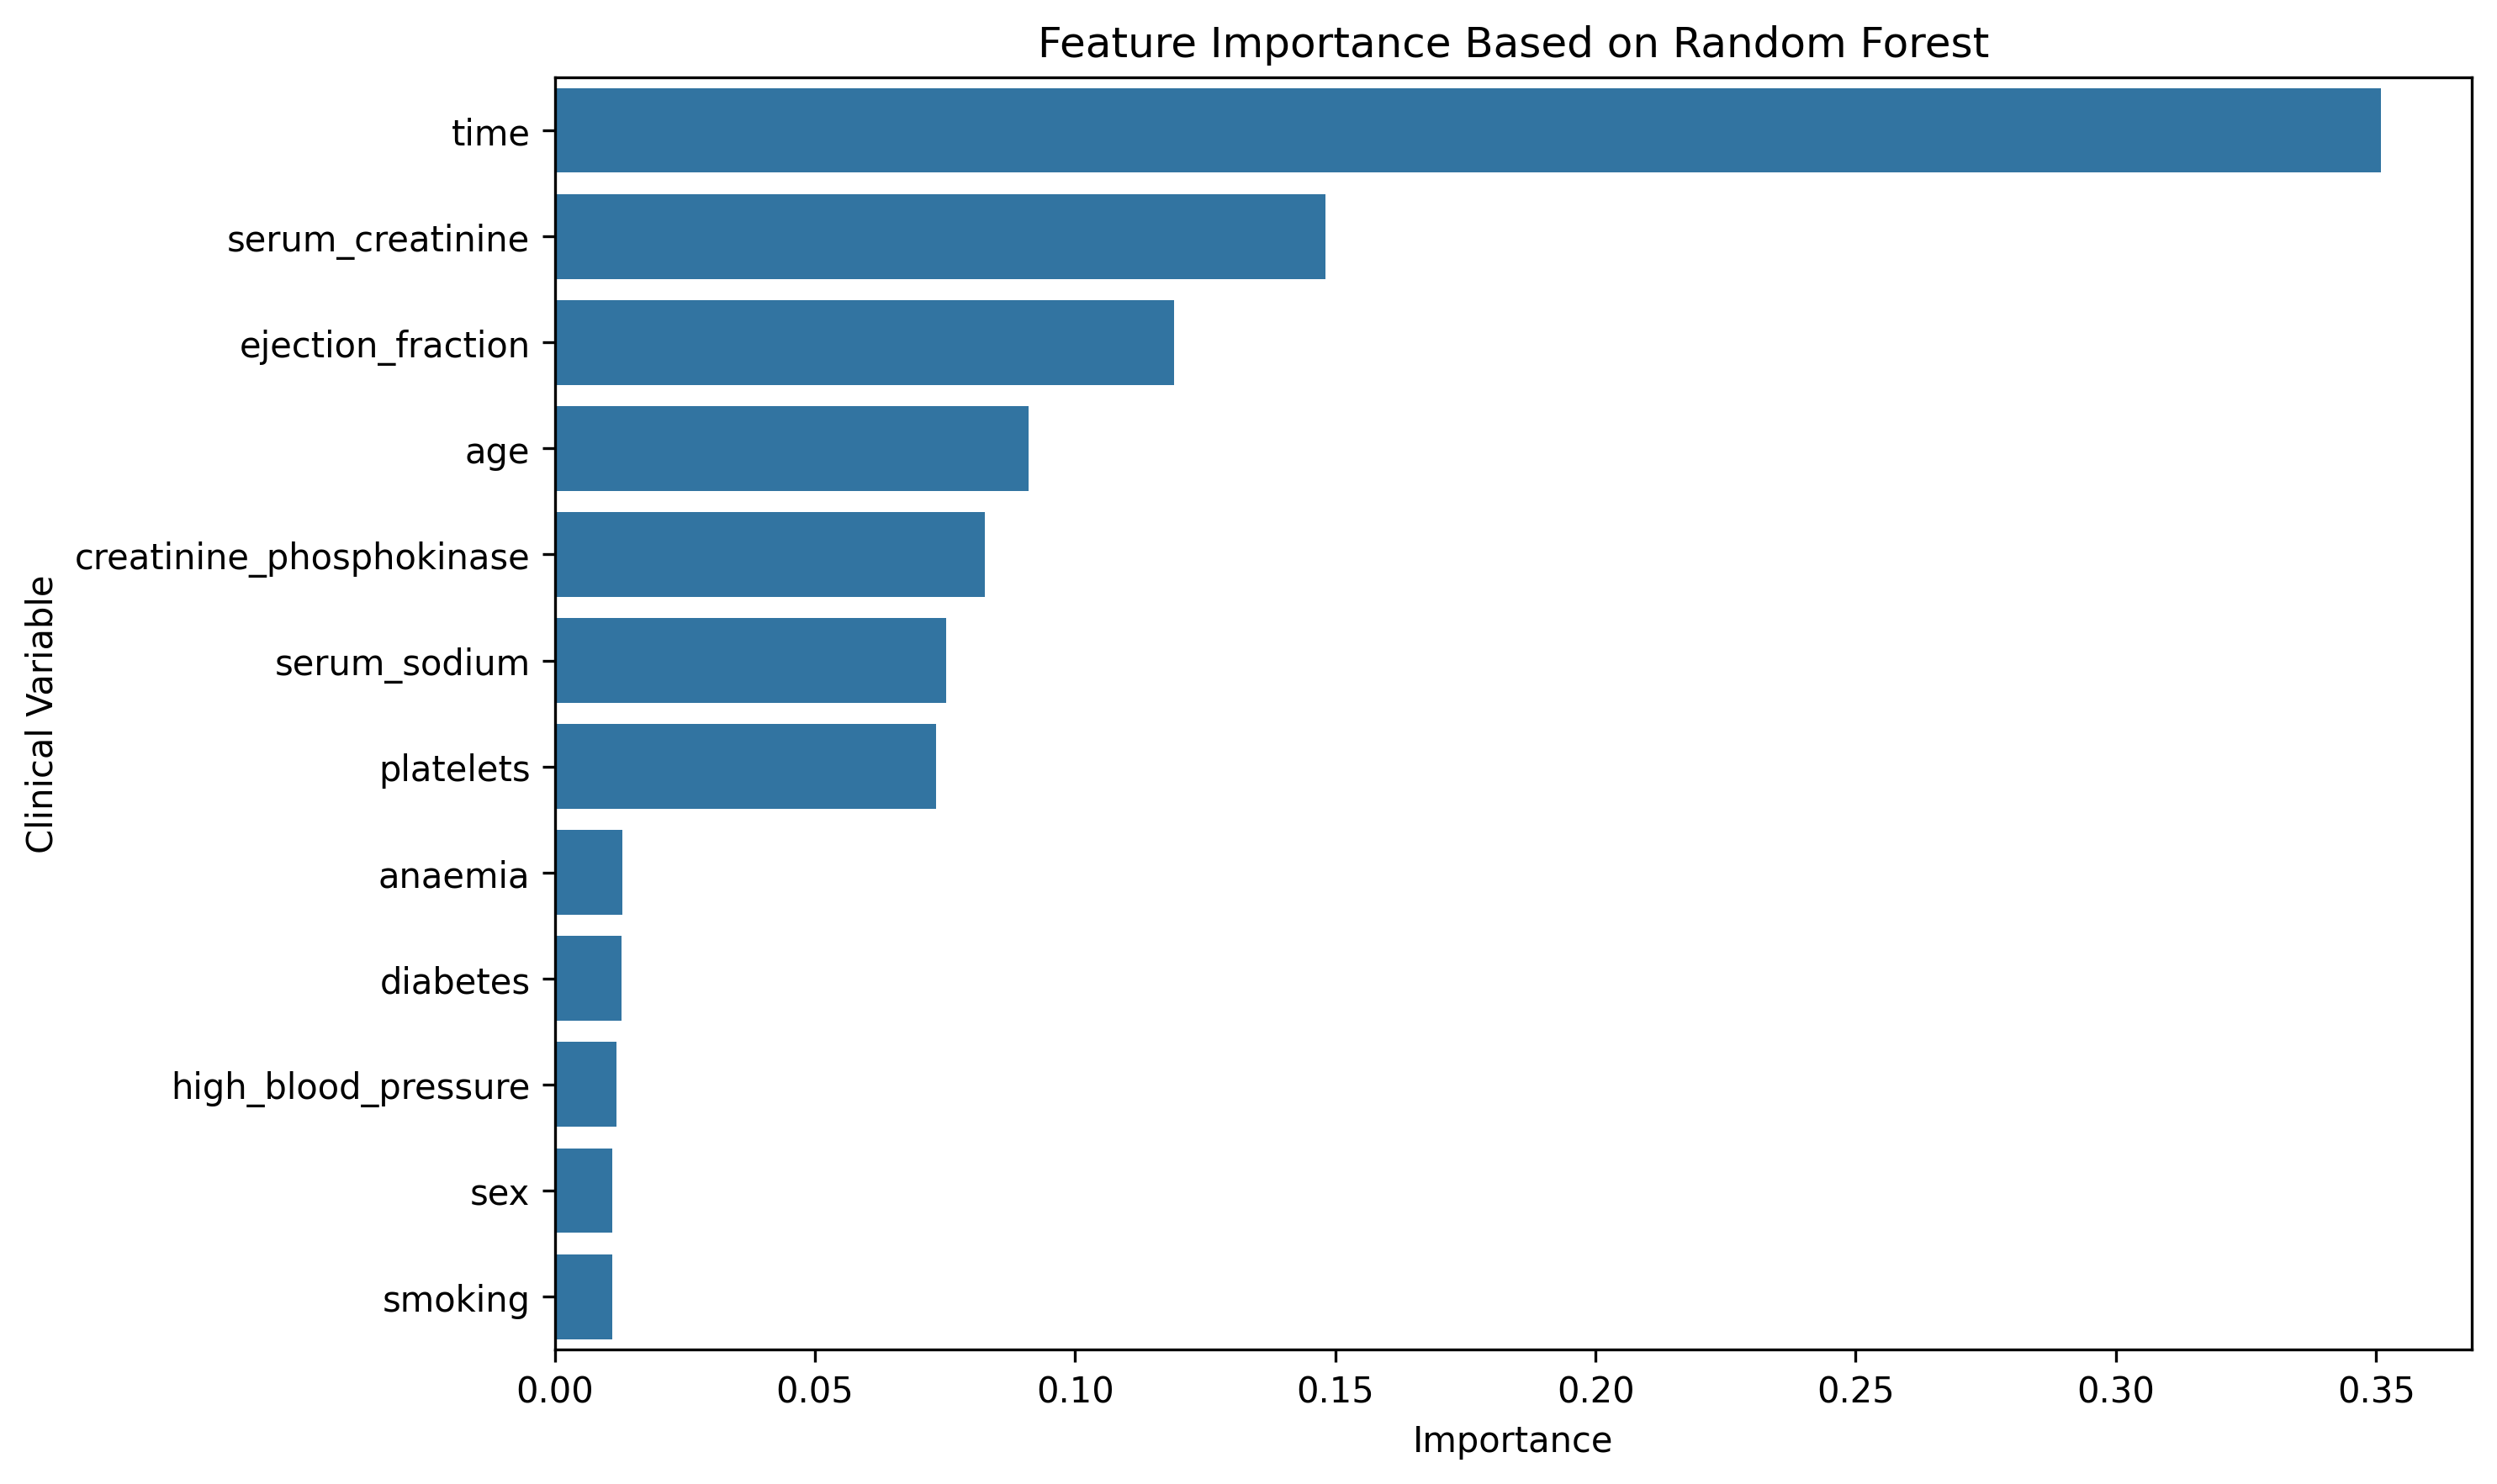
\includegraphics[width=0.85\textwidth]{feature_importance.png}
    \caption{Feature importance scores derived from a Random Forest 
    classifier ($n_\text{estimators} = 500$, \texttt{class\_weight} = 
    ``balanced''). Follow-up time, serum creatinine, and ejection fraction 
    are the three most important predictors, collectively accounting for 
    64.9\% of total importance.}
    \label{fig:importance}
\end{figure}

\subsection{Model Performance}

Table~\ref{tab:performance} summarises the test-set performance of all four 
classifiers. Random Forest achieved the highest AUC (0.897) and F1 score 
(0.727), followed by Logistic Regression (AUC\,=\,0.855). XGBoost matched 
Random Forest in accuracy and F1 but yielded a lower AUC. MLP performed 
below the tree-based models, consistent with the known susceptibility of 
neural networks to small tabular datasets.

\begin{table}[H]
\centering
\caption{Test-set performance of four machine learning classifiers for 
heart failure survival prediction ($n_\text{test} = 60$). Best values in 
each column are highlighted in \textbf{bold}.}
\label{tab:performance}
\renewcommand{\arraystretch}{1.35}
\begin{tabular}{lccccc}
\toprule
\textbf{Model} & \textbf{Accuracy} & \textbf{Precision} & \textbf{Recall} & \textbf{F1 Score} & \textbf{AUC} \\
\midrule
Logistic Regression & 0.800          & 0.733              & 0.579           & 0.647             & 0.855        \\
Random Forest       & \textbf{0.850} & \textbf{0.857}     & \textbf{0.632}  & \textbf{0.727}    & \textbf{0.897} \\
XGBoost             & \textbf{0.850} & \textbf{0.857}     & \textbf{0.632}  & \textbf{0.727}    & 0.849        \\
MLP                 & 0.750          & 0.667              & 0.421           & 0.516             & 0.745        \\
\bottomrule
\end{tabular}
\end{table}

The ROC curves for all four models are displayed in Figure~\ref{fig:roc}. 
Random Forest demonstrated consistently superior sensitivity across most 
operating thresholds. All three traditional ML models (LR, RF, XGBoost) 
substantially outperformed the random-chance baseline, confirming their 
discriminative utility.

\begin{figure}[H]
    \centering
    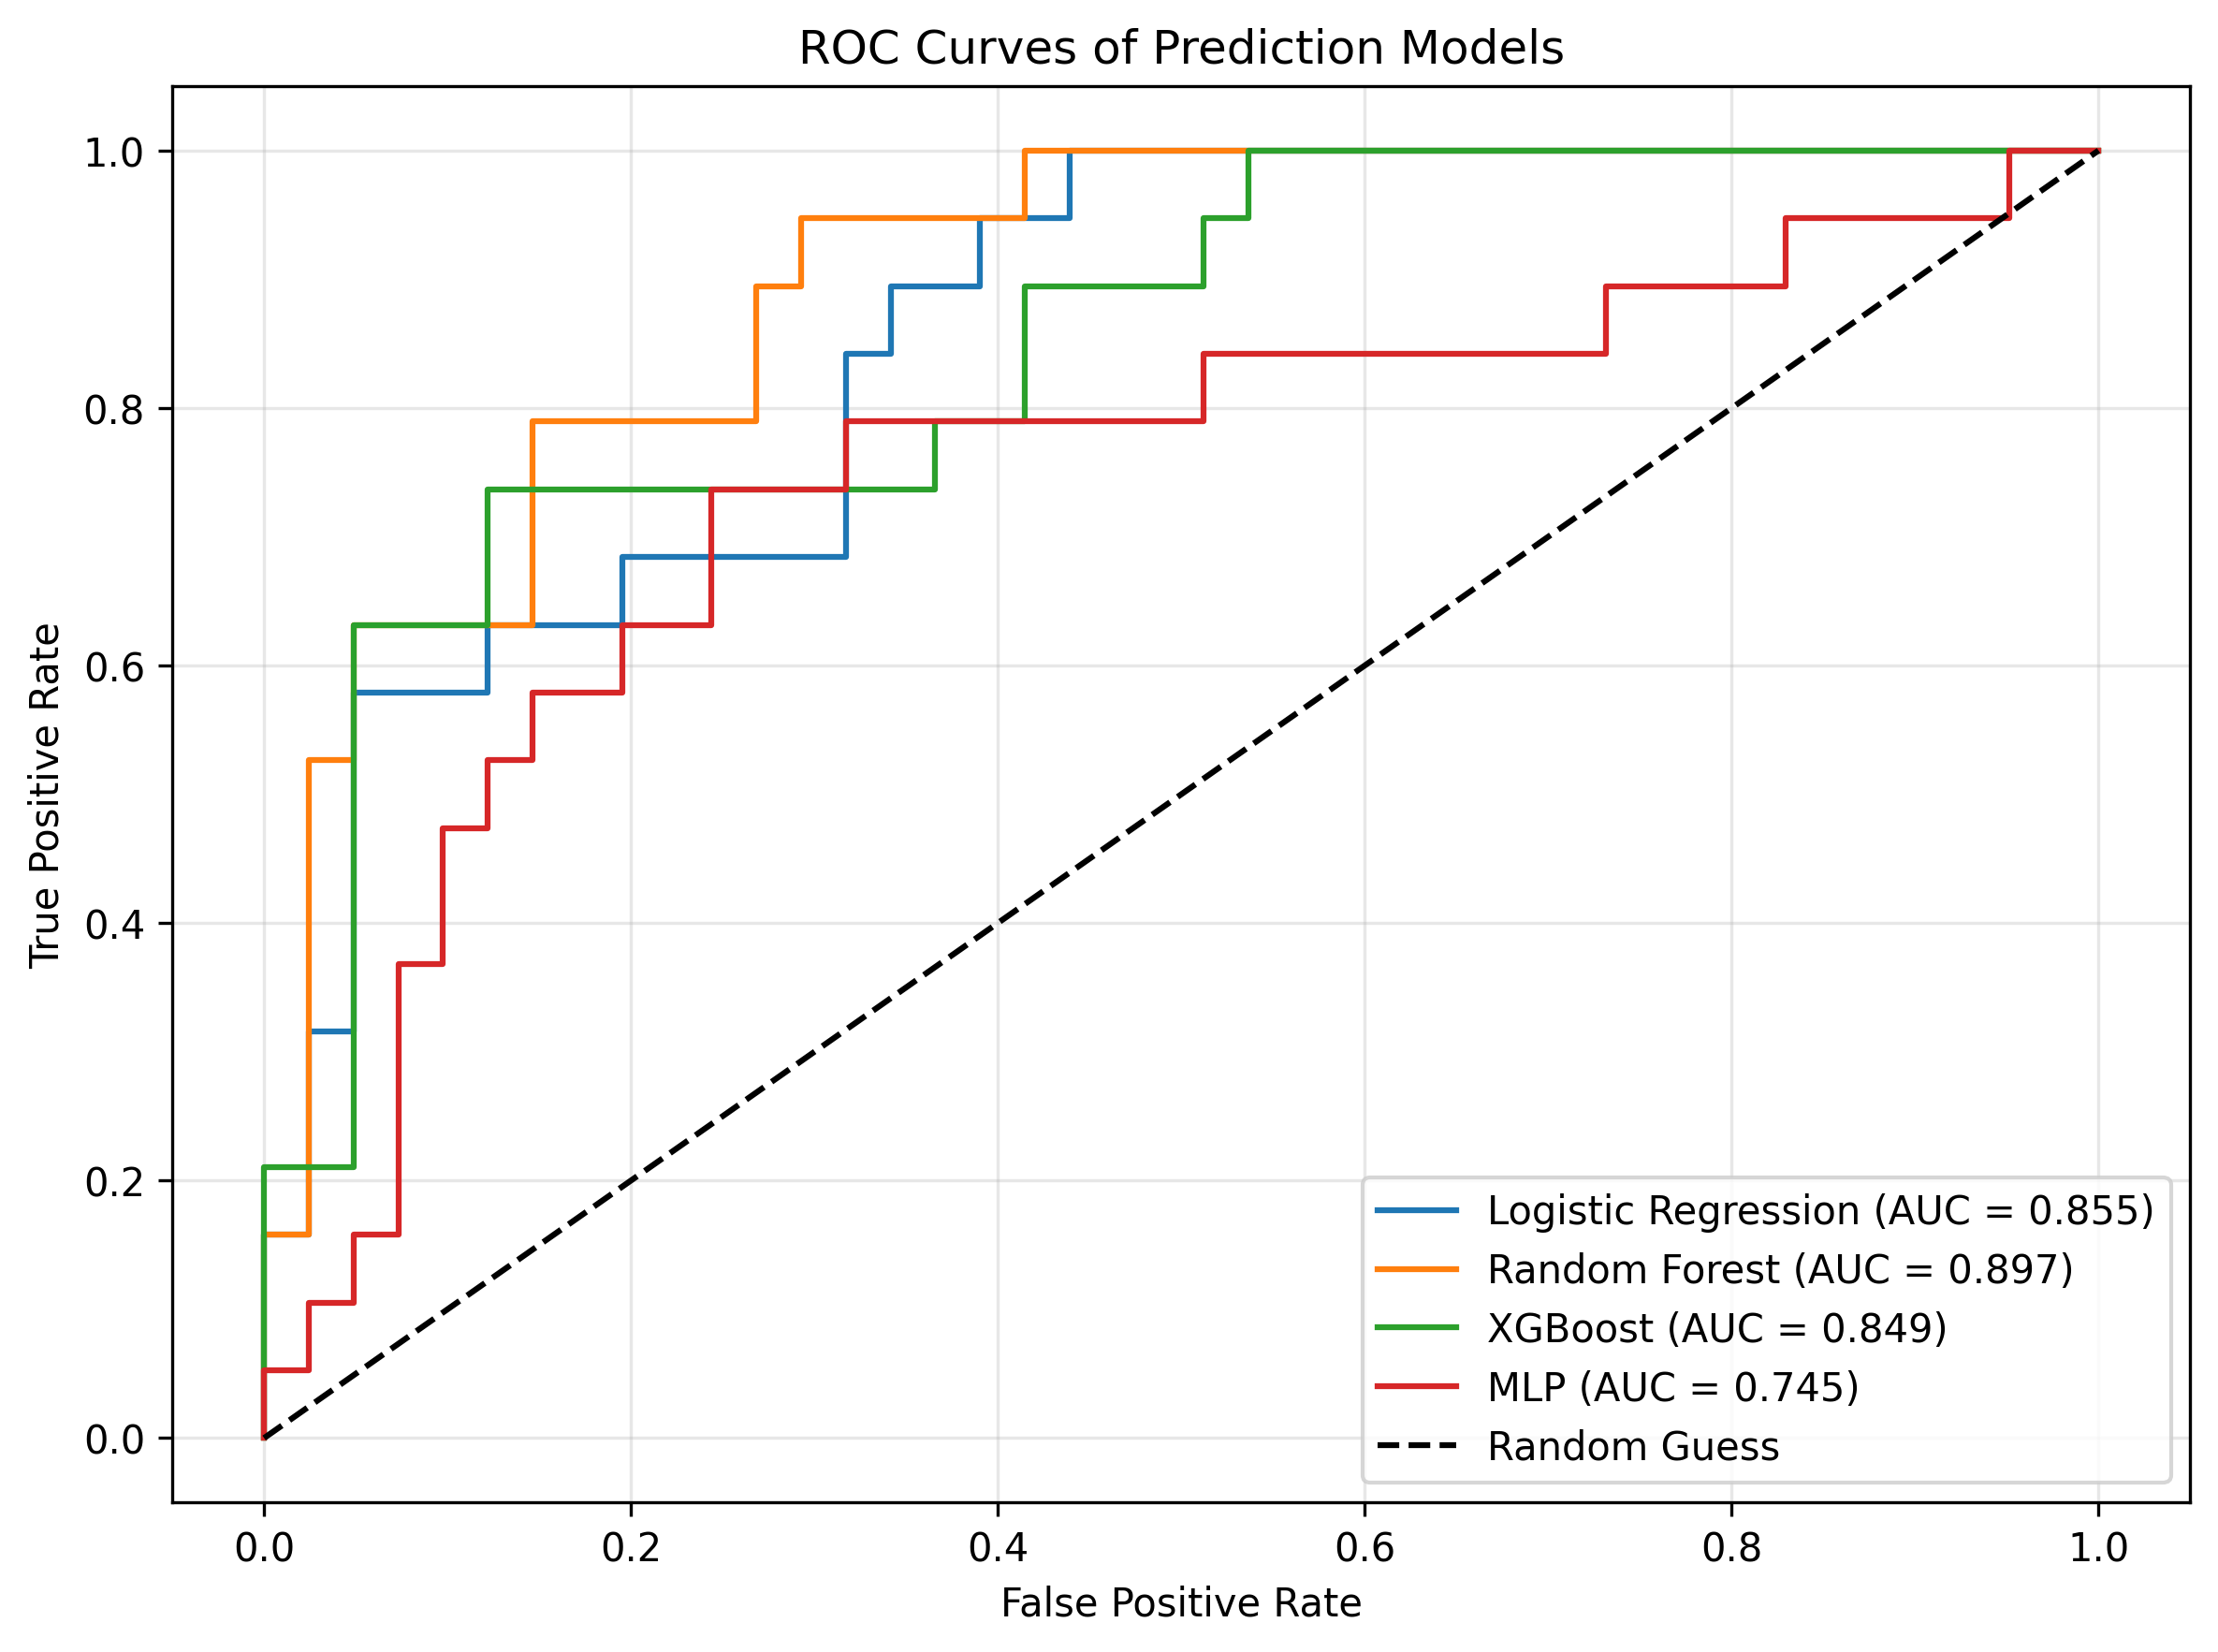
\includegraphics[width=0.80\textwidth]{roc_curve.png}
    \caption{Receiver Operating Characteristic (ROC) curves for four 
    classifiers evaluated on the held-out test set ($n=60$). The dashed 
    diagonal line represents random classification (AUC\,=\,0.5). 
    Random Forest achieves the highest AUC (0.897), followed by 
    Logistic Regression (0.855), XGBoost (0.849), and MLP (0.745).}
    \label{fig:roc}
\end{figure}
\clearpage
\begin{figure}[!htbp]
    \centering
    % ── Replace with your AI-generated workflow figure ──────────────────
    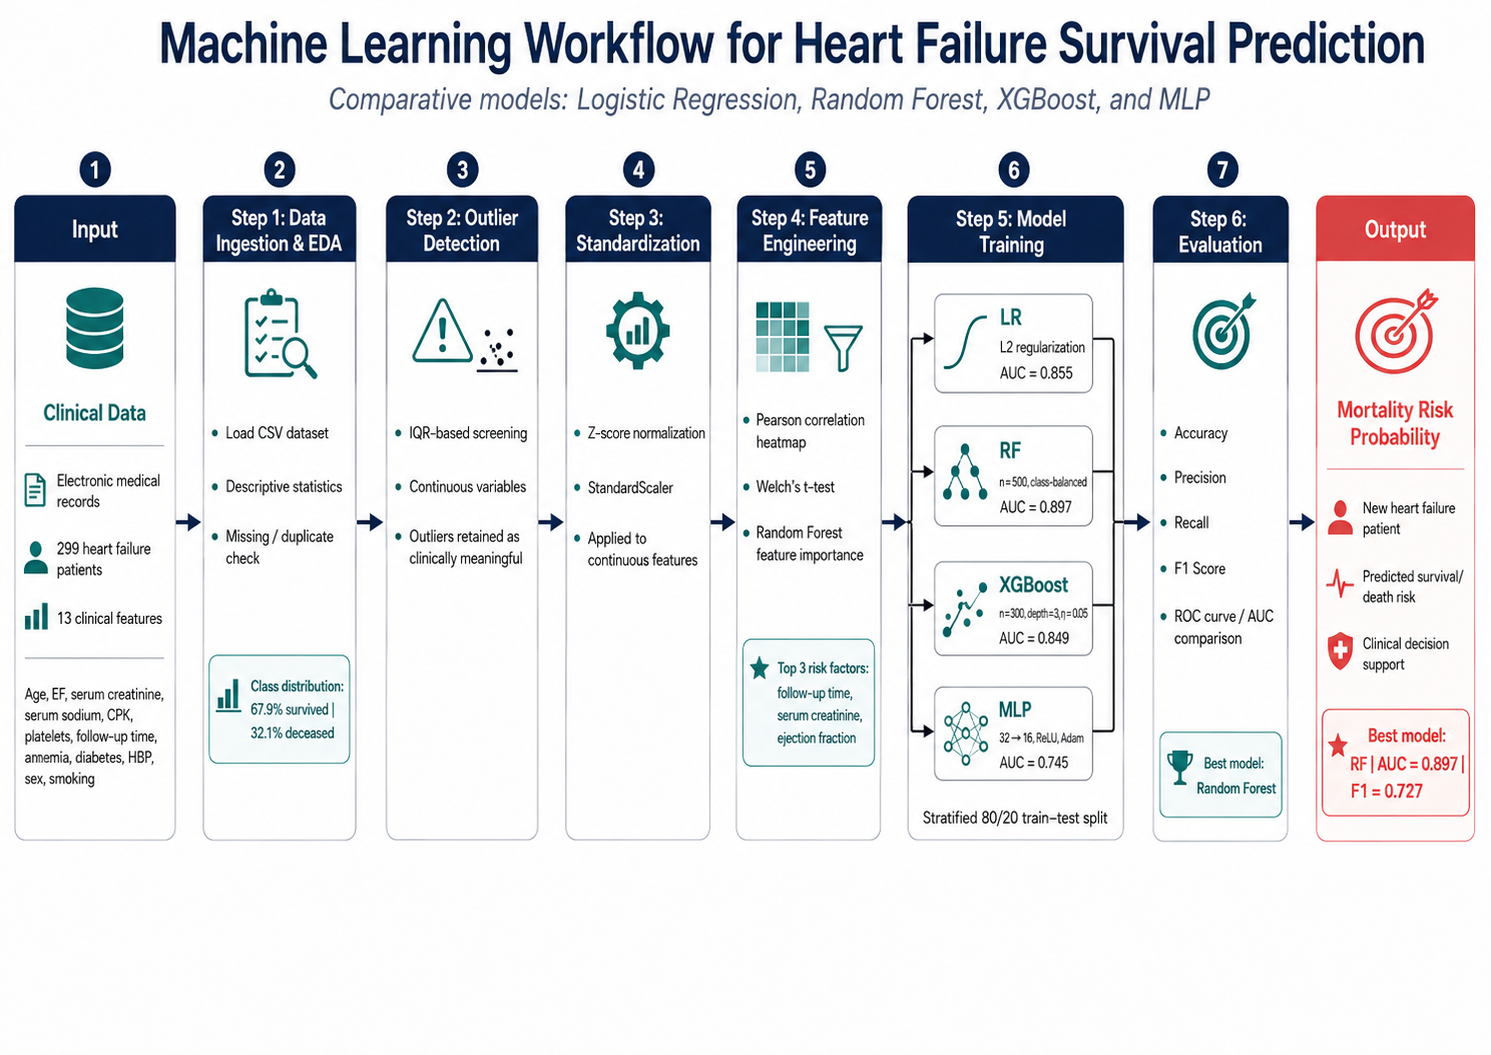
\includegraphics[width=0.88\textwidth]{workflow.png}
    \caption{AI-generated conceptual diagram of the heart failure survival 
    prediction pipeline. The workflow encompasses data ingestion from 
    electronic health records, preprocessing and feature engineering, 
    parallel model training (Logistic Regression, Random Forest, XGBoost, 
    MLP), and comparative evaluation via standardised performance metrics.}
    \label{fig:workflow}
\end{figure}

% ══════════════════════════════════════════════════════════════════════════════
\section{Discussion}
\label{sec:discussion}

\subsection{Principal Findings}

This study demonstrates that ensemble tree-based methods—particularly Random 
Forest—outperform linear and deep learning baselines for short-term mortality 
prediction in heart failure patients using a small, structured clinical 
dataset. Our findings corroborate and extend those of Chicco and 
Jurman \cite{chicco2020}, who reported that serum creatinine and 
ejection fraction are the dominant predictors in this cohort.

The consistently high importance of \textbf{serum creatinine} across both 
statistical and model-based rankings reflects the central role of 
cardiorenal syndrome in HF pathophysiology. Renal dysfunction, indexed by 
elevated creatinine, reduces diuretic responsiveness, promotes neurohormonal 
activation, and independently predicts adverse outcomes in HF \cite{damman2014}.

\textbf{Ejection fraction} is the cornerstone of HF classification. Patients 
with ejection fraction below 40\%—classified as HFrEF—have impaired systolic 
function and substantially worse prognosis than those with preserved ejection 
fraction \cite{ponikowski2016}. The strong negative correlation between EF 
and mortality in our cohort ($r = -0.269$, $p < 0.001$) is entirely 
consistent with this clinical understanding.

\textbf{Follow-up time} warrants special interpretive caution. Although it 
ranks as the strongest predictor in our feature importance analysis, this 
variable is not a conventional clinical biomarker but rather a temporal 
covariate that encodes the censoring structure of the survival data. Its 
inclusion in classification models risks \emph{data leakage}—patients who die 
necessarily have shorter follow-up. In a prospective clinical deployment, 
follow-up time would not be available at the prediction timepoint and should 
therefore be excluded or handled via survival analysis methods such as 
Cox regression \cite{ahmad2017}.

\subsection{Performance Comparison}

Random Forest achieved an AUC of 0.897, consistent with the upper range 
reported in the literature for this dataset (0.75--0.90) \cite{chicco2020, hu2021}. 
The comparable performance of Logistic Regression (AUC\,=\,0.855) highlights 
that linear models remain competitive when features are carefully selected, 
offering the additional advantage of interpretability via odds ratios.

The relative underperformance of MLP (AUC\,=\,0.745) is expected given the 
limited sample size ($n=299$). Deep learning models typically require large 
datasets ($n \geq 10{,}000$) to outperform well-tuned traditional 
algorithms \cite{shwartz2022}. Regularisation strategies (dropout, 
$L_2$ penalty, early stopping) partially mitigated overfitting but could 
not fully compensate for data scarcity.

\subsection{Limitations}

Several limitations should be acknowledged. First, the cohort of 299 patients 
from a single Pakistani centre may not generalise to other populations or 
healthcare settings. Second, class imbalance (67.9\% survivors) may inflate 
accuracy while suppressing recall for the minority (deceased) class; 
strategies such as SMOTE oversampling or threshold calibration were not 
applied. Third, as discussed above, the inclusion of follow-up time as a 
predictor may constitute data leakage in a prospective application. Future 
work should validate these models on independent, multi-centre cohorts and 
explore survival modelling frameworks that appropriately handle censored 
observations.

% ══════════════════════════════════════════════════════════════════════════════
\section{Conclusions}
\label{sec:conclusions}

We conducted a comprehensive machine learning analysis of 299 heart failure 
patients, comparing four classifiers for all-cause mortality prediction. 
Random Forest achieved the best discriminative performance (AUC\,=\,0.897, 
F1\,=\,0.727) and is recommended as the primary model for this task. Feature 
analysis consistently identified follow-up time, serum creatinine, and 
ejection fraction as the most informative predictors, with the latter two 
carrying direct clinical interpretability as biomarkers of cardiorenal and 
cardiac systolic dysfunction, respectively. These results support the 
feasibility of integrating machine learning prognostic tools into routine 
heart failure management, with the caveat that prospective validation in 
larger, diverse cohorts is an essential prerequisite for clinical deployment.

% ══════════════════════════════════════════════════════════════════════════════
\section*{Acknowledgements}
The author thanks the original data collectors \cite{ahmad2017} for making 
the dataset publicly available, and acknowledges the use of AI language model 
assistance (Claude, Anthropic) for code generation and manuscript drafting 
during this project.

\section*{Data Availability}
The Heart Failure Clinical Records dataset is publicly available from the UCI 
Machine Learning Repository: 
\url{https://archive.ics.uci.edu/dataset/519/heart+failure+clinical+records}

% ══════════════════════════════════════════════════════════════════════════════
% Vancouver numbered style matching BMC Medical Informatics
\bibliographystyle{unsrtnat}
\begin{thebibliography}{99}

\bibitem{who2021}
World Health Organization.
\newblock Cardiovascular diseases ({CVDs}): Key facts [Internet]. 2021
  [cited 2026 May 18].
\newblock Available from:
  \url{https://www.who.int/news-room/fact-sheets/detail/cardiovascular-diseases-(cvds)}

\bibitem{virani2021}
Virani SS, Alonso A, Aparicio HJ, Benjamin EJ, Bittencourt MS, Callaway CW,
  et al.
\newblock Heart disease and stroke statistics---2021 update: a report from the
  {American Heart Association}.
\newblock \emph{Circulation}. 2021;143(8):e254--e743.
\newblock \href{https://doi.org/10.1161/CIR.0000000000000950}{doi:10.1161/CIR.0000000000000950}

\bibitem{groenewegen2020}
Groenewegen A, Rutten FH, Mosterd A, Hoes AW.
\newblock Epidemiology of heart failure.
\newblock \emph{Eur J Heart Fail}. 2020;22(8):1342--56.
\newblock \href{https://doi.org/10.1002/ejhf.1858}{doi:10.1002/ejhf.1858}

\bibitem{raphael2007}
Raphael C, Briscoe C, Davies J, Whinnett ZI, Manisty C, Sutton R, et al.
\newblock Limitations of the {New York Heart Association} functional
  classification system and self-reported walking distances in chronic heart
  failure.
\newblock \emph{Heart}. 2007;93(4):476--82.
\newblock \href{https://doi.org/10.1136/hrt.2006.089656}{doi:10.1136/hrt.2006.089656}

\bibitem{chicco2020}
Chicco D, Jurman G.
\newblock Machine learning can predict survival of patients with heart failure
  from serum creatinine and ejection fraction alone.
\newblock \emph{BMC Med Inform Decis Mak}. 2020;20(1):16.
\newblock \href{https://doi.org/10.1186/s12911-020-1023-5}{doi:10.1186/s12911-020-1023-5}

\bibitem{ahmad2017}
Ahmad T, Munir A, Bhatti SH, Aftab M, Raza MA.
\newblock Survival analysis of heart failure patients: a case study.
\newblock \emph{PLoS ONE}. 2017;12(7):e0181001.
\newblock \href{https://doi.org/10.1371/journal.pone.0181001}{doi:10.1371/journal.pone.0181001}

\bibitem{hu2021}
Hu H, Li Z, Yan J, Wang X, Xiao H, Ding Z, et al.
\newblock Survival prediction of heart failure patients using machine learning
  techniques.
\newblock \emph{Inform Med Unlocked}. 2021;26:100772.
\newblock \href{https://doi.org/10.1016/j.imu.2021.100772}{doi:10.1016/j.imu.2021.100772}

\bibitem{damman2014}
Damman K, Testani JM.
\newblock The kidney in heart failure: an update.
\newblock \emph{Eur Heart J}. 2015;36(23):1437--44.
\newblock \href{https://doi.org/10.1093/eurheartj/ehv010}{doi:10.1093/eurheartj/ehv010}

\bibitem{ponikowski2016}
Ponikowski P, Voors AA, Anker SD, Bueno H, Cleland JGF, Coats AJS, et al.
\newblock 2016 {ESC} Guidelines for the diagnosis and treatment of acute and
  chronic heart failure.
\newblock \emph{Eur Heart J}. 2016;37(27):2129--200.
\newblock \href{https://doi.org/10.1093/eurheartj/ehw128}{doi:10.1093/eurheartj/ehw128}

\bibitem{shwartz2022}
Shwartz-Ziv R, Armon A.
\newblock Tabular data: deep learning is not all you need.
\newblock \emph{Inf Fusion}. 2022;81:84--90.
\newblock \href{https://doi.org/10.1016/j.inffus.2021.11.011}{doi:10.1016/j.inffus.2021.11.011}

\end{thebibliography}

\end{document}